\subsection{Der RC-Kreis als Integrator}
In den Abbildungen \ref{fig:Rechteck}, \ref{fig:dreieck} und \ref{fig:Sinus} wird der Zusammenhang als Integrationsglied deutlich.
Aus der Hochfrequenten sinusschwingung (Abb. \ref{fig:Sinus}) entsteht einen um $\pi / 2$ verschobene Schwingung bzw eine Kosinusschwingung.
Die Rechteckspannung (Abb. \ref{fig:Rechteck}) wird zu einer Dreiecksspannung integriert und die Dreieckspannung (Abb. \ref{fig:dreieck}) 
zu einer Folge von Parabelbögen.


\begin{figure}
    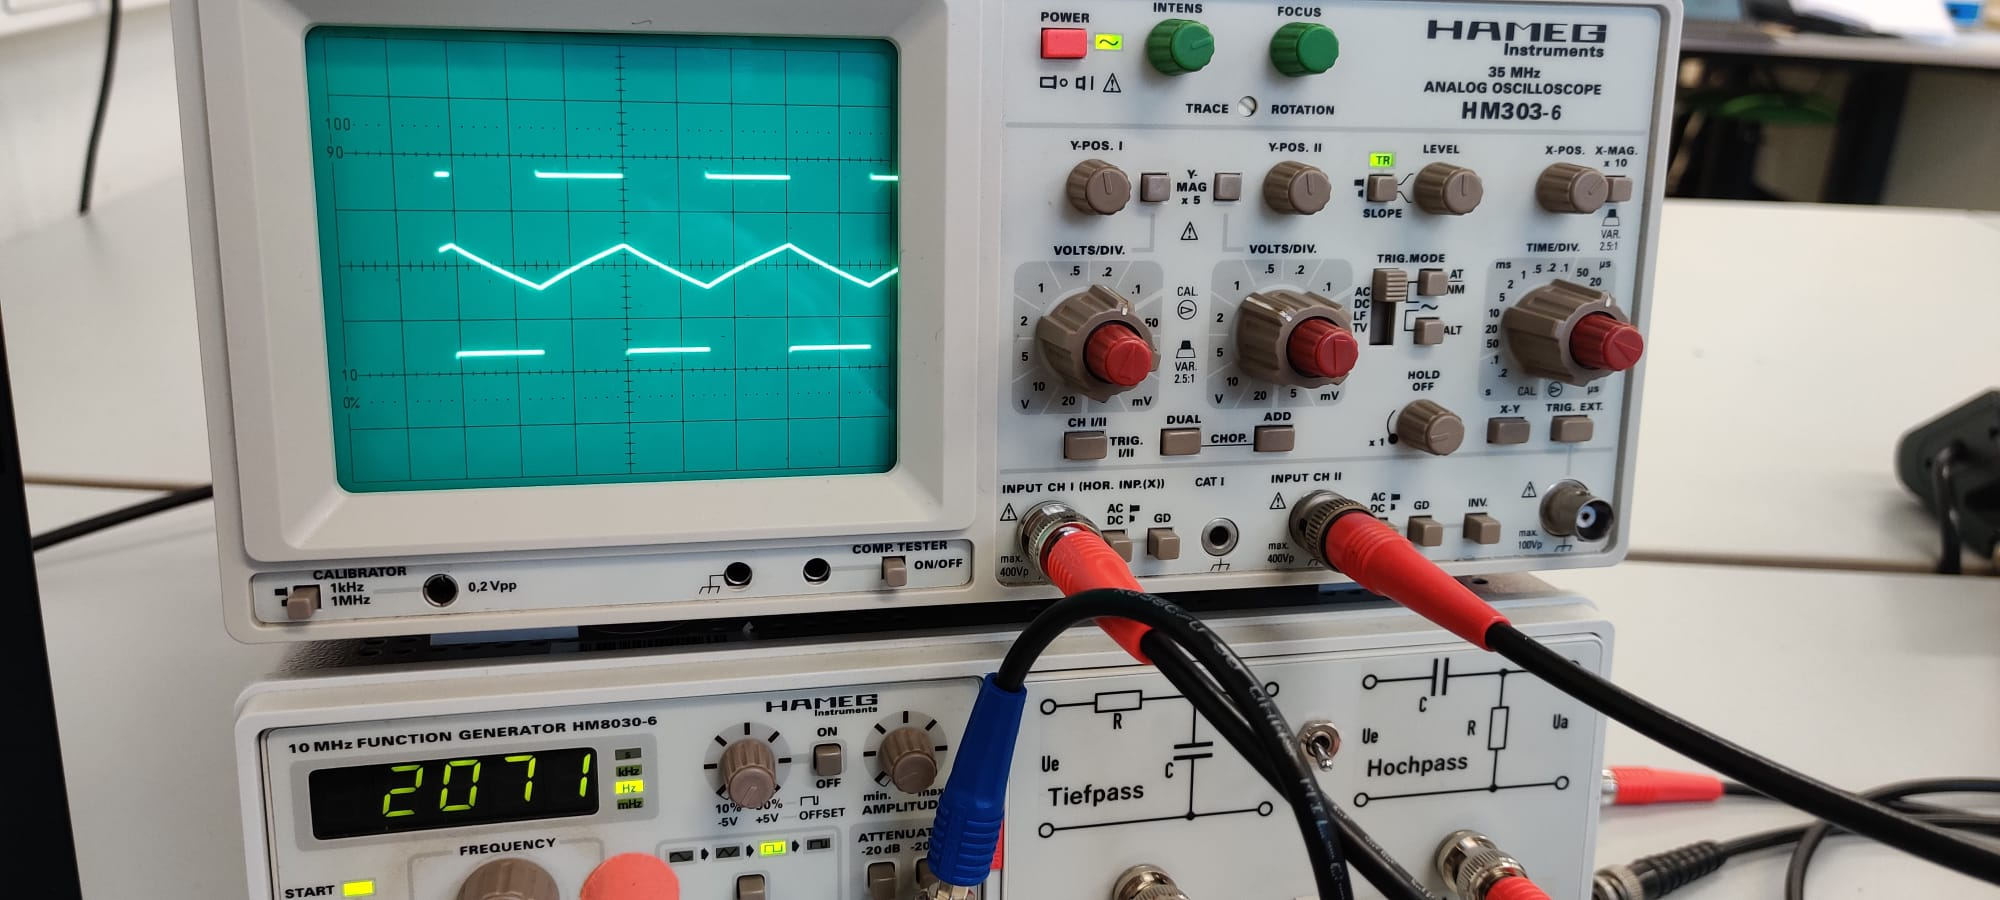
\includegraphics[width=\textwidth]{abbildungen/Rechtecksspannung.jpeg}
    \caption{Rechteckspannung regt Dreieckschwingung.}
    \label{fig:Rechteck}
\end{figure}
\begin{figure}
    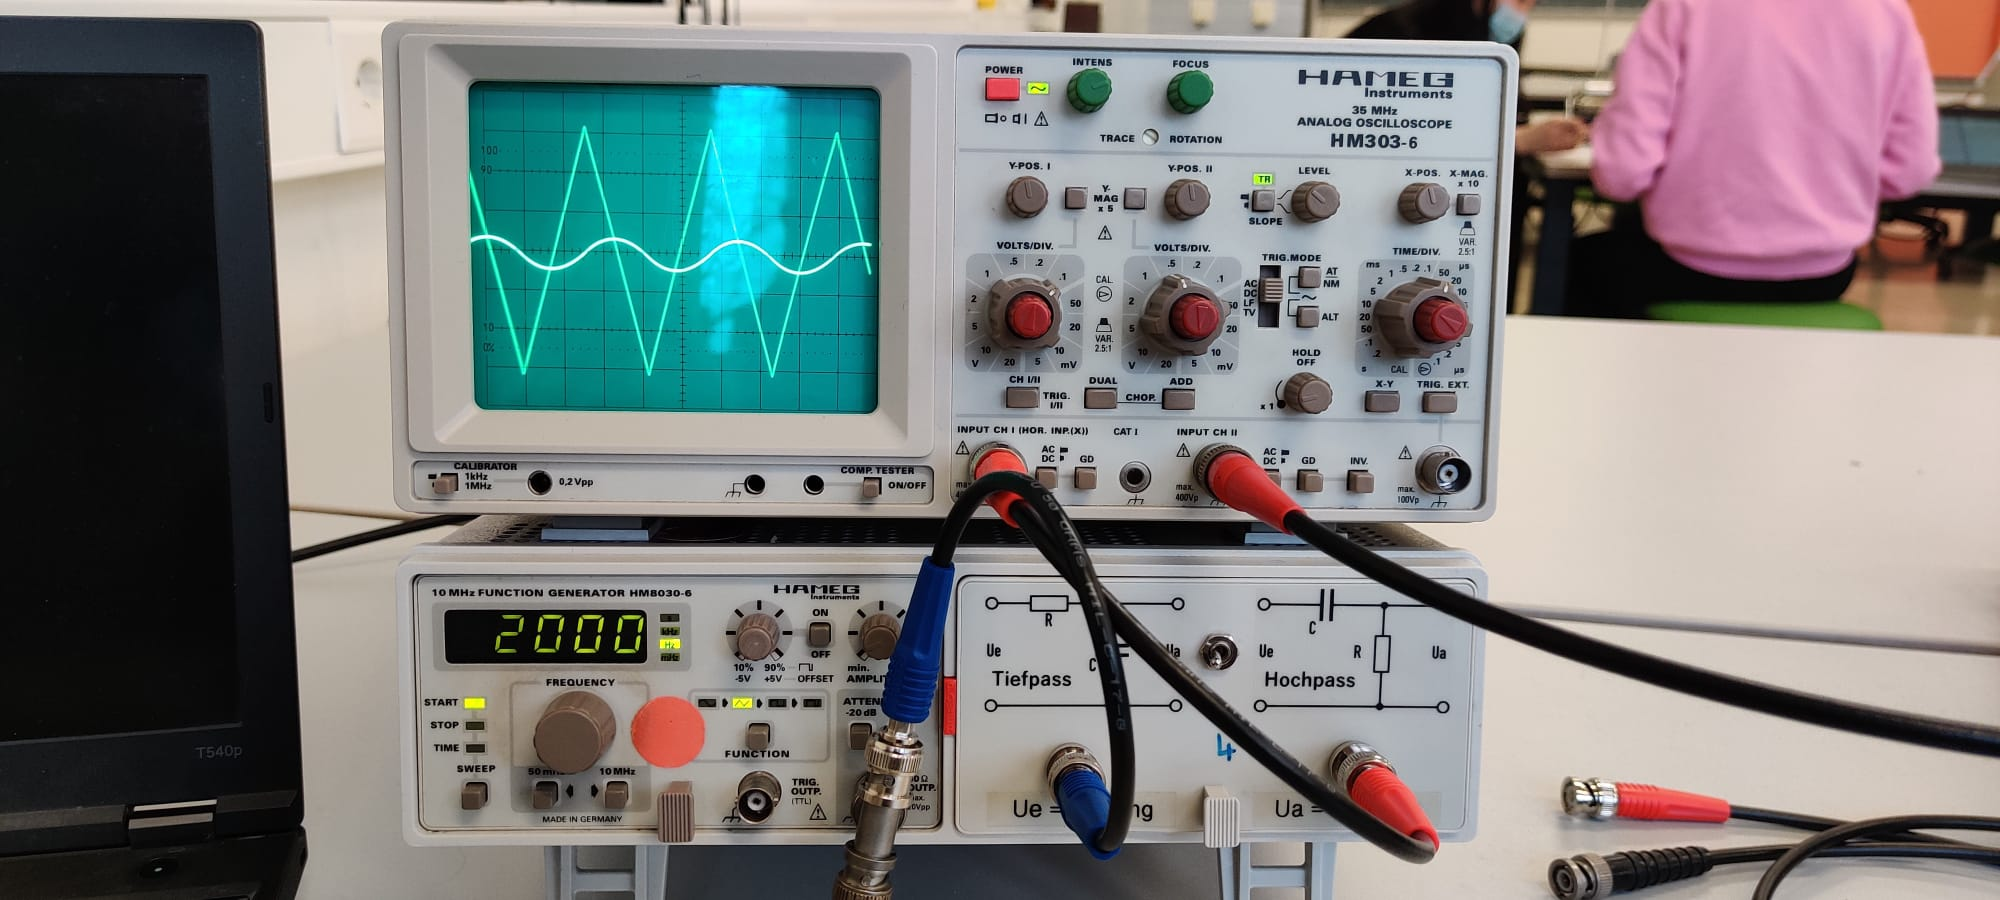
\includegraphics[width=\textwidth]{abbildungen/DreiecksSchwingung.jpeg}
    \caption{Dreiecksschwingung regt Parabelschwingung an.}
    \label{fig:dreieck}
\end{figure}
\begin{figure}
    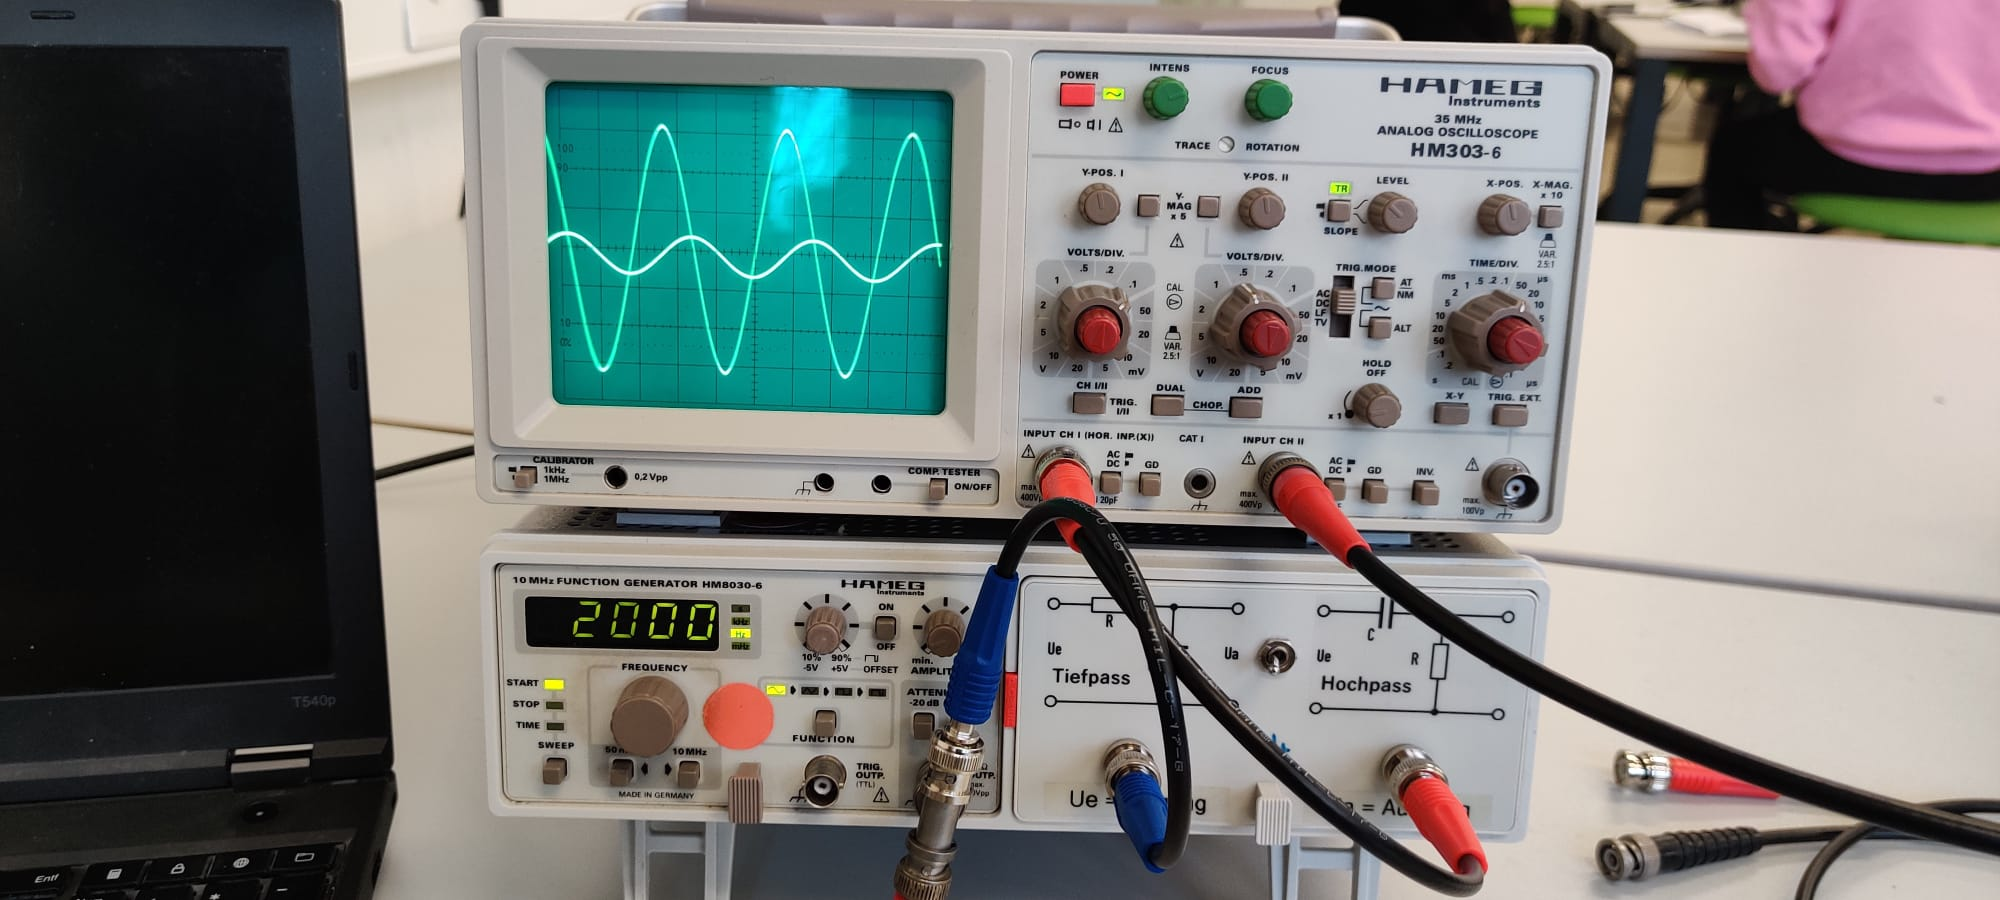
\includegraphics[width=\textwidth]{abbildungen/Sinusschwingung.jpeg}
    \caption{Sinusschwingung regt Kosinusschwingung an.}
    \label{fig:Sinus}
\end{figure}